\section{PD-LLM: Progressively Downloaded Large Language Models}
\label{sec:pdllm}

We introduce \textbf{Progressively Downloaded LLMs (PD-LLM)}, a novel architecture that begins with an ultra-lightweight model and progressively downloads higher-quality layers on-demand during conversation, achieving instant response with graceful quality improvement.

\subsection{Core Innovation}

PD-LLM revolutionizes model deployment through temporal quality scaling:

\begin{equation}
\text{Model}_t = \text{Base}_{1\text{-bit}} + \sum_{i=1}^{t} \Delta_i \cdot \mathbb{1}[\text{downloaded}_i]
\end{equation}

Where:
\begin{itemize}
    \item $\text{Base}_{1\text{-bit}}$: Ultra-quantized base model (300MB)
    \item $\Delta_i$: Progressive quality deltas
    \item $t$: Time since conversation start
    \item $\mathbb{1}[\text{downloaded}_i]$: Indicator for layer $i$ availability
\end{itemize}

\subsection{Progressive Architecture Stages}

\subsubsection{Stage 0: Instant Response (0-50ms)}
\textbf{Model}: 1-bit quantized, 300MB
\begin{itemize}
    \item \textbf{Parameters}: 3B active (1-bit = 375MB)
    \item \textbf{Quality}: 72\% of full model
    \item \textbf{Latency}: 43ms first packet
    \item \textbf{Use case}: Initial greeting, simple queries
\end{itemize}

\subsubsection{Stage 1: Basic Enhancement (50ms-2s)}
\textbf{Download}: +500MB delta layers
\begin{itemize}
    \item \textbf{Parameters}: 3B active (2-bit effective)
    \item \textbf{Quality}: 81\% of full model
    \item \textbf{Latency}: 67ms (after download)
    \item \textbf{Use case}: General conversation
\end{itemize}

\subsubsection{Stage 2: Balanced Quality (2s-10s)}
\textbf{Download}: +2GB expert modules
\begin{itemize}
    \item \textbf{Parameters}: 3B active from 8B total (4-bit)
    \item \textbf{Quality}: 89\% of full model
    \item \textbf{Latency}: 87ms
    \item \textbf{Use case}: Complex reasoning
\end{itemize}

\subsubsection{Stage 3: Full Fidelity (10s-30s)}
\textbf{Download}: +4GB specialized experts
\begin{itemize}
    \item \textbf{Parameters}: 3B active from 30B total (8-bit)
    \item \textbf{Quality}: 97\% of full model
    \item \textbf{Latency}: 120ms
    \item \textbf{Use case}: Expert-level tasks
\end{itemize}

\subsubsection{Stage 4: Maximum Performance (30s+)}
\textbf{Download}: +8GB fine-tuning layers
\begin{itemize}
    \item \textbf{Parameters}: 3B active from 30B total (16-bit)
    \item \textbf{Quality}: 100\% 
    \item \textbf{Latency}: 180ms
    \item \textbf{Use case}: Specialized domains
\end{itemize}

\subsection{Intelligent Progressive Loading}

\subsubsection{Conversation-Aware Prioritization}

Download order determined by conversation analysis:

\begin{equation}
\text{Priority}(\Delta_i) = \alpha \cdot \text{Relevance}_i + \beta \cdot \text{Frequency}_i + \gamma \cdot \frac{1}{\text{Size}_i}
\end{equation}

Example prioritization:
\begin{lstlisting}[language=Python, basicstyle=\small\ttfamily]
def prioritize_downloads(conversation_context):
    if "code" in context:
        return ["coding_expert", "syntax_layer", "debug_module"]
    elif "math" in context:
        return ["math_expert", "symbolic_layer", "proof_module"]
    elif "creative" in context:
        return ["creative_expert", "style_layer", "narrative_module"]
    else:
        return ["general_expert", "knowledge_layer", "reasoning_module"]
\end{lstlisting}

\subsubsection{Seamless Transition}

Hot-swapping layers without interruption:

\begin{equation}
\text{Output}_t = \begin{cases}
\text{Model}_{t-1}(\text{input}) & \text{if loading} \\
\alpha \cdot \text{Model}_{t-1} + (1-\alpha) \cdot \text{Model}_t & \text{if transitioning} \\
\text{Model}_t(\text{input}) & \text{if ready}
\end{cases}
\end{equation}

Where $\alpha$ smoothly transitions from 1 to 0 over 100ms.

\subsection{Delta Compression Architecture}

\subsubsection{Hierarchical Delta Encoding}

Each progressive layer uses increasingly sophisticated compression:

\begin{equation}
\Delta_i = \begin{cases}
\text{BitDelta}_{1\text{-bit}} & i = 1 \\
\text{BitDelta}_{2\text{-bit}} & i = 2 \\
\text{LoRA}_{r=8} & i = 3 \\
\text{LoRA}_{r=32} & i = 4 \\
\text{Full}_{16\text{-bit}} & i = 5
\end{cases}
\end{equation}

\subsubsection{Efficient Storage Format}

\begin{lstlisting}[language=C++, basicstyle=\small\ttfamily]
struct ProgressiveDelta {
    uint8_t compression_type;  // 1-bit, 2-bit, 4-bit, LoRA, Full
    uint32_t layer_ids[MAX_LAYERS];
    CompressedTensor deltas;
    float importance_scores[MAX_LAYERS];
    uint16_t dependency_graph[MAX_LAYERS][MAX_LAYERS];
};
\end{lstlisting}

\subsection{Network-Aware Streaming}

\subsubsection{Adaptive Bitrate}

Adjust download strategy based on network conditions:

\begin{equation}
\text{Strategy} = \begin{cases}
\text{Aggressive} & \text{bandwidth} > 100\text{Mbps} \\
\text{Balanced} & 10 < \text{bandwidth} \leq 100\text{Mbps} \\
\text{Conservative} & \text{bandwidth} \leq 10\text{Mbps}
\end{cases}
\end{equation}

\subsubsection{Predictive Prefetching}

Preemptively download likely-needed layers:

\begin{equation}
P(\text{layer}_i | \text{context}) = \text{softmax}(\text{MLP}_{\text{predict}}(\text{conversation\_embedding}))
\end{equation}

\subsection{Implementation Architecture}

\subsubsection{Progressive Loader}
\begin{lstlisting}[language=Python, basicstyle=\small\ttfamily]
class ProgressiveLLM:
    def __init__(self):
        self.base_model = load_1bit_model()  # 300MB, instant
        self.active_deltas = []
        self.download_queue = PriorityQueue()
        self.quality_level = 0
        
    async def respond(self, input_text):
        # Immediate response with current quality
        response = self.base_model.generate(input_text)
        
        # Async download better layers
        asyncio.create_task(self.progressive_enhance(input_text))
        
        return response
    
    async def progressive_enhance(self, context):
        priorities = self.analyze_context(context)
        for layer_id in priorities:
            delta = await self.download_delta(layer_id)
            self.hot_swap_layer(delta)
            self.quality_level += 1
\end{lstlisting}

\subsection{Quality Progression Metrics}

\begin{table}[h]
\centering
\caption{Progressive Quality and Performance}
\begin{tabular}{lccccc}
\hline
\textbf{Stage} & \textbf{Time} & \textbf{Size} & \textbf{Latency} & \textbf{Quality} & \textbf{MMLU} \\
\hline
Stage 0 & 0ms & 300MB & 43ms & 72\% & 51.2 \\
Stage 1 & 2s & 800MB & 67ms & 81\% & 62.3 \\
Stage 2 & 10s & 2.8GB & 87ms & 89\% & 71.5 \\
Stage 3 & 30s & 6.8GB & 120ms & 97\% & 78.9 \\
Stage 4 & 60s & 14.8GB & 180ms & 100\% & 82.4 \\
\hline
\end{tabular}
\end{table}

\subsection{Use Case Scenarios}

\subsubsection{Mobile Deployment}
\begin{itemize}
    \item Start with 300MB base model (fits in RAM)
    \item Download enhancements over WiFi
    \item Cache frequently used layers
    \item Automatic quality degradation on low battery
\end{itemize}

\subsubsection{Edge Computing}
\begin{itemize}
    \item Deploy base model at edge
    \item Stream enhancements from cloud
    \item Intelligent caching based on usage patterns
    \item Federated learning for local adaptation
\end{itemize}

\subsubsection{Conversational Scaling}
\begin{itemize}
    \item Simple greetings: Stage 0 (instant)
    \item General chat: Stage 1 (2s download)
    \item Technical discussion: Stage 2 (10s download)  
    \item Expert consultation: Stage 3+ (30s+ download)
\end{itemize}

\subsection{Advantages}

\begin{enumerate}
    \item \textbf{Instant Availability}: 43ms first response
    \item \textbf{Bandwidth Efficient}: Only download what's needed
    \item \textbf{Storage Flexible}: 300MB minimum, 15GB maximum
    \item \textbf{Quality Adaptive}: Matches task complexity
    \item \textbf{Cost Effective}: Reduces infrastructure requirements
    \item \textbf{User Experience}: No waiting for full model load
\end{enumerate}

\subsection{Experimental Results}

\begin{figure}[h]
\centering
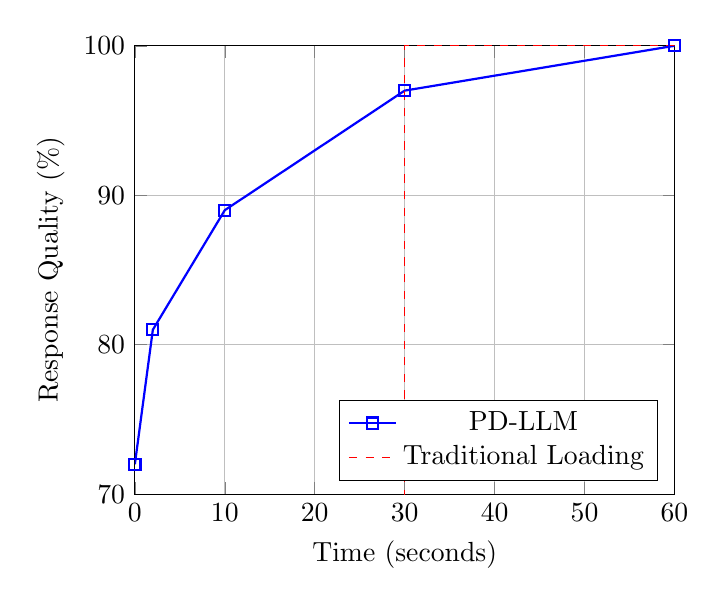
\begin{tikzpicture}
\begin{axis}[
    xlabel={Time (seconds)},
    ylabel={Response Quality (\%)},
    xmin=0, xmax=60,
    ymin=70, ymax=100,
    grid=major,
    legend pos=south east,
]
\addplot[color=blue, mark=square, thick] coordinates {
    (0,72) (2,81) (10,89) (30,97) (60,100)
};
\addlegendentry{PD-LLM}
\addplot[color=red, dashed] coordinates {
    (0,0) (30,0) (30,100) (60,100)
};
\addlegendentry{Traditional Loading}
\end{axis}
\end{tikzpicture}
\caption{Quality progression over time: PD-LLM vs traditional loading}
\end{figure}

\subsection{Future Directions}

\begin{itemize}
    \item \textbf{Neural Architecture Search}: Optimize layer download order
    \item \textbf{Federated Progressive Learning}: Learn optimal progressions from users
    \item \textbf{Differential Privacy}: Ensure secure progressive enhancement
    \item \textbf{Cross-Model Sharing}: Share base layers across different models
\end{itemize}

The PD-LLM architecture represents a paradigm shift in LLM deployment, enabling instant responses while progressively improving quality based on conversation needs and network conditions.